\documentclass[11pt,a4paper]{article}
\usepackage[margin=2.3cm]{geometry}
\usepackage{amsmath,amssymb,graphicx,booktabs,hyperref,xcolor,caption,float}
\usepackage[T1]{fontenc}
\hypersetup{colorlinks=true,linkcolor=blue!50!black,urlcolor=blue!50!black,citecolor=blue!50!black}
\captionsetup{font=small,labelfont=bf}
\graphicspath{{../../plots/pquasar_diagnostics/}}
\newcommand{\code}[1]{\texttt{#1}}
\newcommand{\pq}{p_{\rm quasar}}

\title{Two weaknesses of $\pq$:\\ unranked quasars and top-end overconfidence}
\author{Internal note, \code{qso\_pcolor}}
\date{4 October 2026}

\begin{document}
\maketitle

\section*{Summary}
\begin{itemize}
\item \textbf{Unranked quasars.} Of 38,881 held-out test quasars above the faint limit, the scorer declines to
  rank 2.9\% with model A (magnitude-dependent, \code{current}) and 3.2\% with model B (magnitude-independent,
  \code{current\_magindep}). For 89--92\% of them the reason is \emph{outside both models}: the colours are more
  than $4\sigma$ from both the quasar and the background model. The rest fail the QSO-support cut.
\item \textbf{The cause is mainly the $4\sigma$ test, not the quasars.} The distance is a raw Mahalanobis distance
  in each object's observed bands, and it grows with the number of bands $k$, while the cut is fixed. The
  unranked fraction is 0\% for $k<12$, 0.4--0.9\% for $k=13$--15, 2--4\% for $k=17$--19 and 7--15\% for $k\ge20$.
  The unranked quasars continue the distance distribution of the ranked ones just past the cut
  (Figs.~\ref{fig:dist}, \ref{fig:k}).
\item Rescored with Legacy $g,r,z,W1,W2$ only, 93--94\% of them are ranked; removing any one large survey (SDSS,
  PS1, AllWISE or the Legacy WISE bands) rescues 56--85\%. No single survey or band is responsible.
  A secondary contribution is disagreement between surveys observed at different epochs (quasar variability):
  $|r_{\rm SDSS}-r_{\rm Legacy}|>0.5$\,mag for 33\% of unranked quasars and 11\% of ranked ones.
\item \textbf{Fix (implemented, validated, the default since 5 October 2026):} calibrate the same distance statistic per object
  by simulating members of each class model in the object's own bands with its own noise
  (Section~\ref{sec:fix}). On the test panel, quasars outside both models fall from 2.5--2.9\% to 0.14--0.17\% and
  unranked quasars from 2.9--3.2\% to 0.6\%, with no dependence on the number of bands; background incidence at
  $\pq>0.5$ changes by $+0.05$ percentage points. (A plain $\chi^2_k$ conversion over-corrects: 2 of 38,881 quasars
  would remain flagged, because the distance is to the nearest of many mixture components.)
\item \textbf{Top-end overconfidence is mostly a labelling effect.} In the natural test-cone population, objects
  with $\pq>0.97$ are known quasars in 58--72\% of cases (lower bound), but 171 of the 188 background objects
  there are already flagged as likely quasars (WISE AGN colours or Quaia). Counting those as quasars gives
  0.93--0.99 (upper bound), close to the predicted values. Only 17 of the 188 are unflagged, 1.7--2.9\% of
  all objects at $\pq>0.97$ after weighting. The model's top end is at most mildly overconfident; better
  labels, not a recalibration, would settle by how much.
\end{itemize}

\section{Data and definitions}
\paragraph{When the scorer declines to rank.} After the faint limit (Legacy $r$ $S/N\ge10$), an object is not
ranked if (i) it is \emph{outside both models}, i.e.\ its Mahalanobis distance to the nearest component of the
quasar model at any redshift, $d_Q$, and to the nearest component of the background model, $d_B$, both exceed
\code{ood\_flag\_sigma}$\,=4$; or (ii) it fails the \emph{QSO-support cut}: the percentile of its colour density
under the quasar model at the primary's redshift is below $2/256$. Both are computed in the object's observed
bands. Unranked objects get no $\pq$ and no ranking statistic.

\paragraph{Samples.}
\begin{itemize}
\item \emph{Test panel} (Part~1): the main performance panel of the method note, 2$\times$20,000 random held-out
  (role 3) quasars per hemisphere with their actual band coverage, of which 38,881 pass the faint limit. They
  were scored by both promoted bundles (the bundle files are identical to the promoted ones). That run used
  support threshold $6/256$; we re-apply the promoted $2/256$ from the stored percentiles.
\item \emph{Natural population} (Part~2): the calibration test of the method note (Section~10.6): all 1,640
  known spectroscopic quasars in the 49 held-out test cones above the faint limit, and 40,000 of the cones'
  background objects weighted by 2.75 to restore their natural share. The background sample still holds
  unidentified quasars; 1,443 of the 40,000 are flagged as likely quasars (Quaia membership, or Legacy
  $W1-W2>0.8$ Vega).
\end{itemize}
Script: \code{scripts/method\_unified/pquasar\_diagnostics.py}; numbers in \code{pquasar\_diagnostics.json}.

%======================================================================
\section{Part 1: real quasars left unranked}
%======================================================================
\subsection{How many, and why}
\begin{center}
\begin{tabular}{lrr}
\toprule
& A (magnitude-dependent) & B (magnitude-independent) \\
\midrule
Test quasars & 38,881 & 38,881 \\
Unranked & 1,113 (2.9\%) & 1,235 (3.2\%) \\
\quad outside both models & 989 & 1,132 \\
\quad QSO-support cut & 118 & 97 \\
\quad no quasar prior at this magnitude & 6 & 6 \\
\bottomrule
\end{tabular}
\end{center}
806 quasars are unranked by both models, 307 by A only and 429 by B only. In the smaller natural sample of the
method note the rates are 3.8\% (A) and 3.5\% (B), from about 60 objects.

\subsection{Who they are}
Figure~\ref{fig:frac} shows the unranked fraction against the quasars' properties. It is flat in redshift
(2.3--3.4\% for $0.5<z<3.25$; 5\% below $z=0.5$) and rises to 7.5--15\% above $z=3.25$ (few quasars, where the
quasar model is sparsest). In magnitude it is lowest at $r=19$--20 for model A (1.2\%) and highest at $r=21$--22.5 (3.7--3.9\%);
model B is worse than A for bright quasars ($r<19$: 2.8--5.5\% against 1.3--2.8\%), where its single colour
width per redshift fits worst. It does not depend on extinction or Galactic latitude. The strongest trend is
with the number of observed bands: 0.5--1.1\% for 10--15 bands, 2.2\% for 16--17, 3.9\% for 18--19, 8.3\% for
20--21, 10.5\% for 22--23 and 20\% for 24--25 (45 quasars).

\begin{figure}[H]\centering
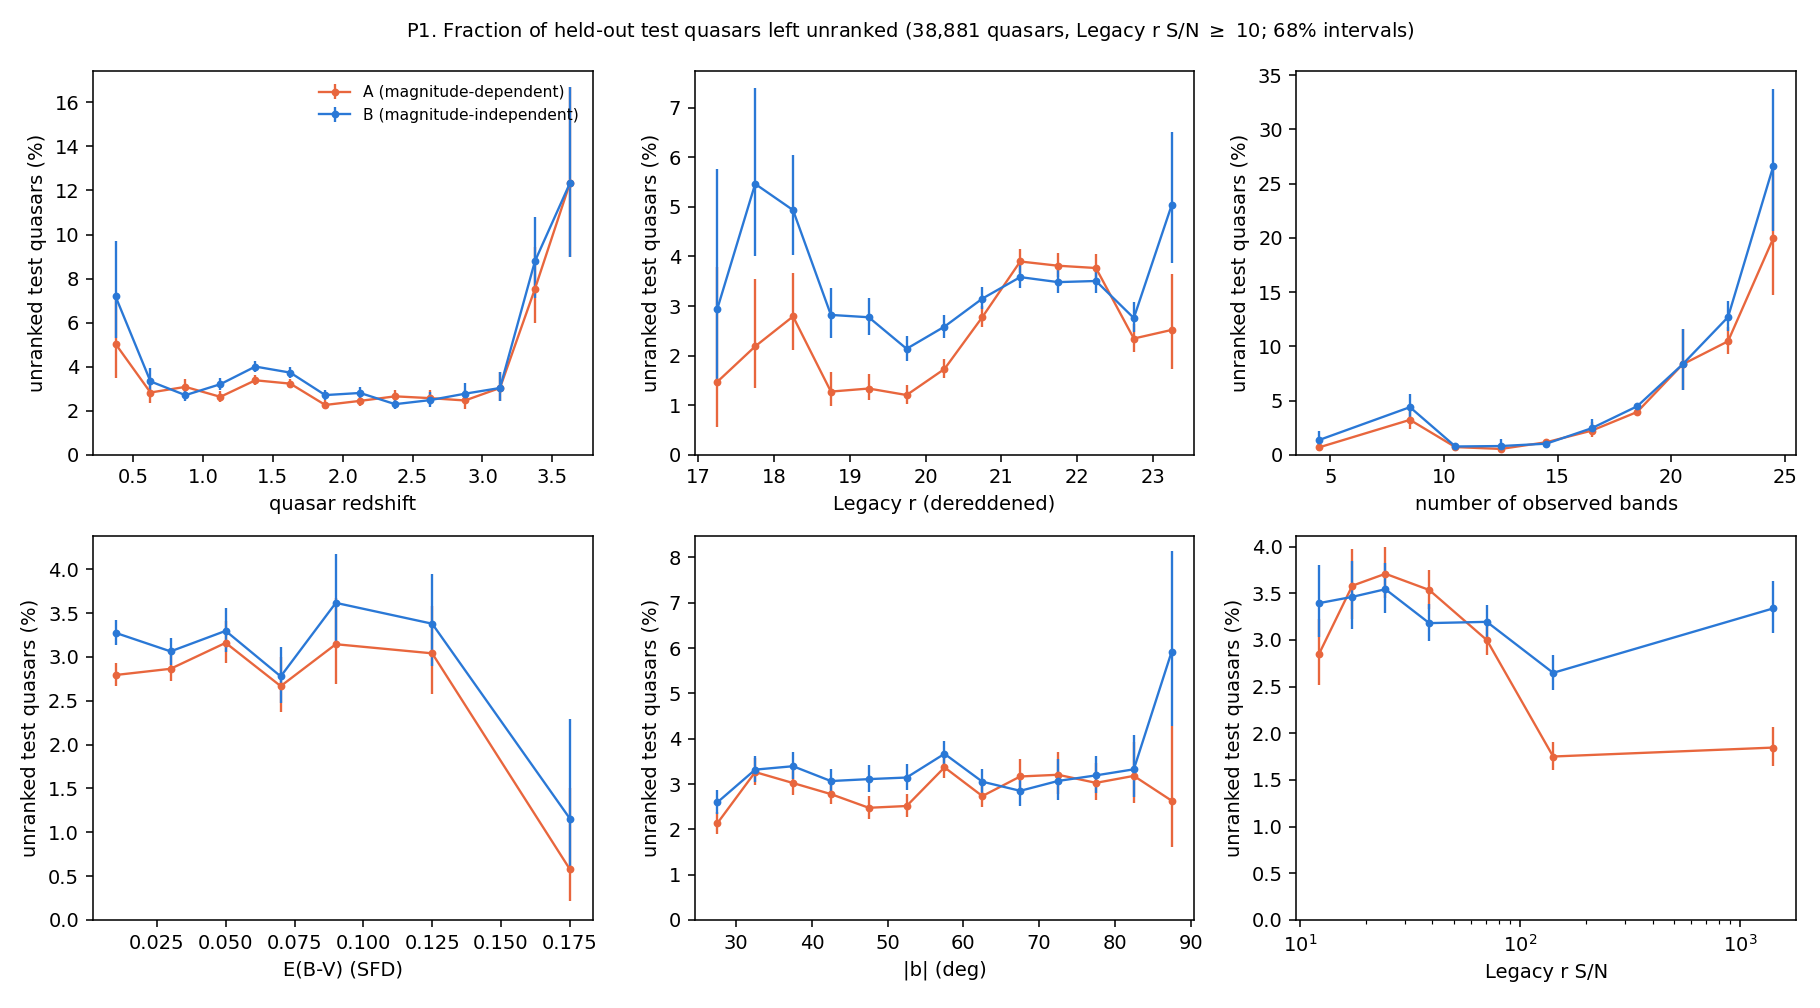
\includegraphics[width=\textwidth]{P1_unranked_fraction.png}
\caption{Fraction of held-out test quasars left unranked, against redshift, Legacy $r$, number of observed
bands, $E(B-V)$, $|b|$ and Legacy $r$ signal-to-noise, for models A (orange) and B (blue). Bars: 68\% Wilson
intervals; bins with fewer than 30 quasars are omitted.}
\label{fig:frac}
\end{figure}

\subsection{They sit just past the cut}
Figure~\ref{fig:dist} places every test quasar by its two distances. Ranked quasars fill a continuous cloud up to
$d_Q=4$; the outside-both-models quasars are its continuation, with $d_Q$ mostly between 4 and 6. They are the
tail of the same population, not a separate group of strange objects. Support-rejected quasars lie inside the
cloud in $d_Q$: they are close to \emph{some} quasar component, but not to the quasar model at their own redshift.

\begin{figure}[H]\centering
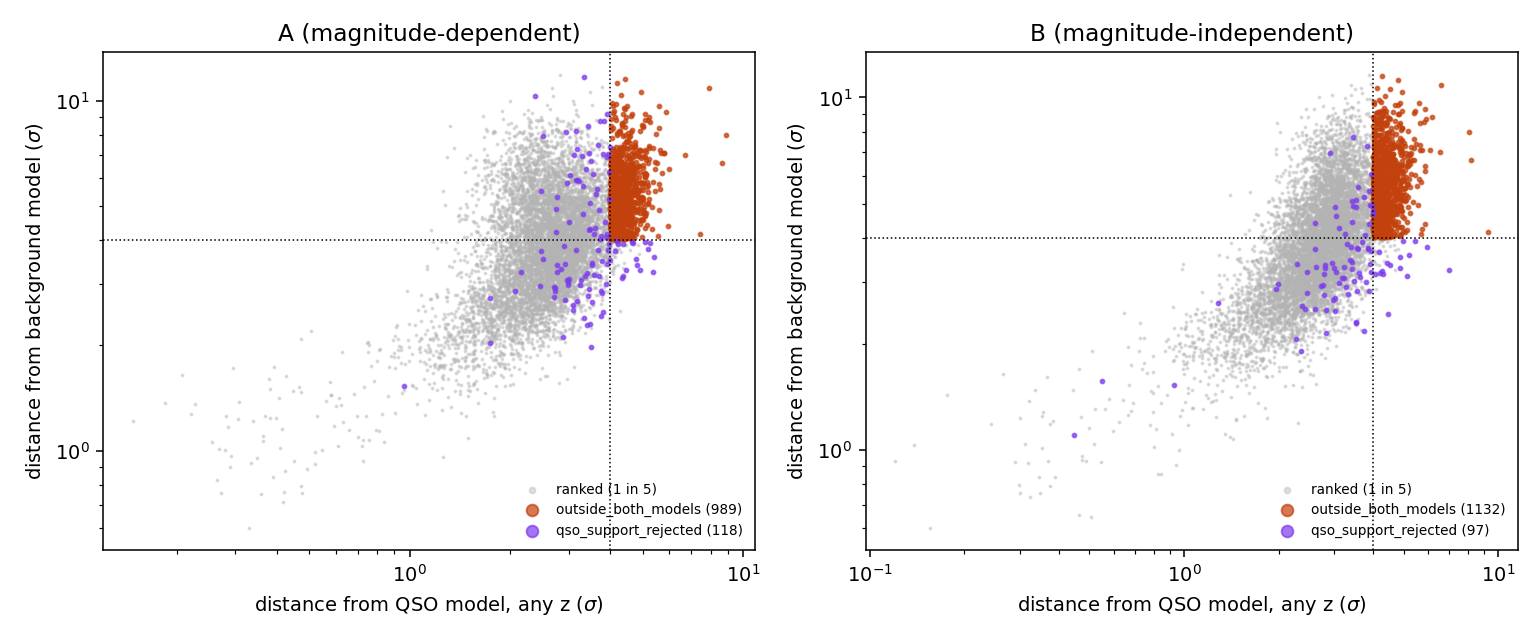
\includegraphics[width=\textwidth]{P2_distances.png}
\caption{Distance from the quasar model at any redshift ($d_Q$) against distance from the background model
($d_B$), in $\sigma$, for test quasars: ranked (grey, one in five), outside both models (orange) and
support-rejected (purple). Dotted: the $4\sigma$ cut on each.}
\label{fig:dist}
\end{figure}

\subsection{The cause: the distance grows with the number of bands}
For a Gaussian in $k$ dimensions the squared Mahalanobis distance of a member follows $\chi^2_k$, whose median
is about $k$; a typical member lies at $d\approx\sqrt{k}$, i.e.\ $3.2\sigma$ at $k=10$ and $4.5\sigma$ at $k=20$.
A fixed cut at $4\sigma$ is therefore strict for objects with many bands and loose for objects with few. The code
documents this (the distance ``is a different tail probability in 3 and in 4 dimensions'') but the cut does not
correct for it. Figure~\ref{fig:k} shows the effect in the data. The median $d_Q$ of test quasars rises from
1.8 at $k=10$ to 3.3 at $k=23$, and its 99th percentile crosses 4 at $k\approx14$. The fraction outside both
models rises in step: 0\% for $k\le12$, 0.4--0.9\% for $k=13$--15, 2--4\% for $k=17$--19, 7--10\% for $k=20$--22
and 15\% at $k=23$. Background objects show the same rise, from at most 0.2\% for $10\le k\le13$ to 16--18\% at $k\ge26$.
The distance grows more slowly than $\sqrt{\chi^2_k}$ because it is measured to the nearest of many mixture
components, so the textbook $\chi^2_k$ correction overshoots: converted to an equivalent Gaussian
significance with $k$ degrees of freedom, only 2 (A) and 1 (B) of the 38,881 test quasars would remain outside
both models.

\begin{figure}[H]\centering
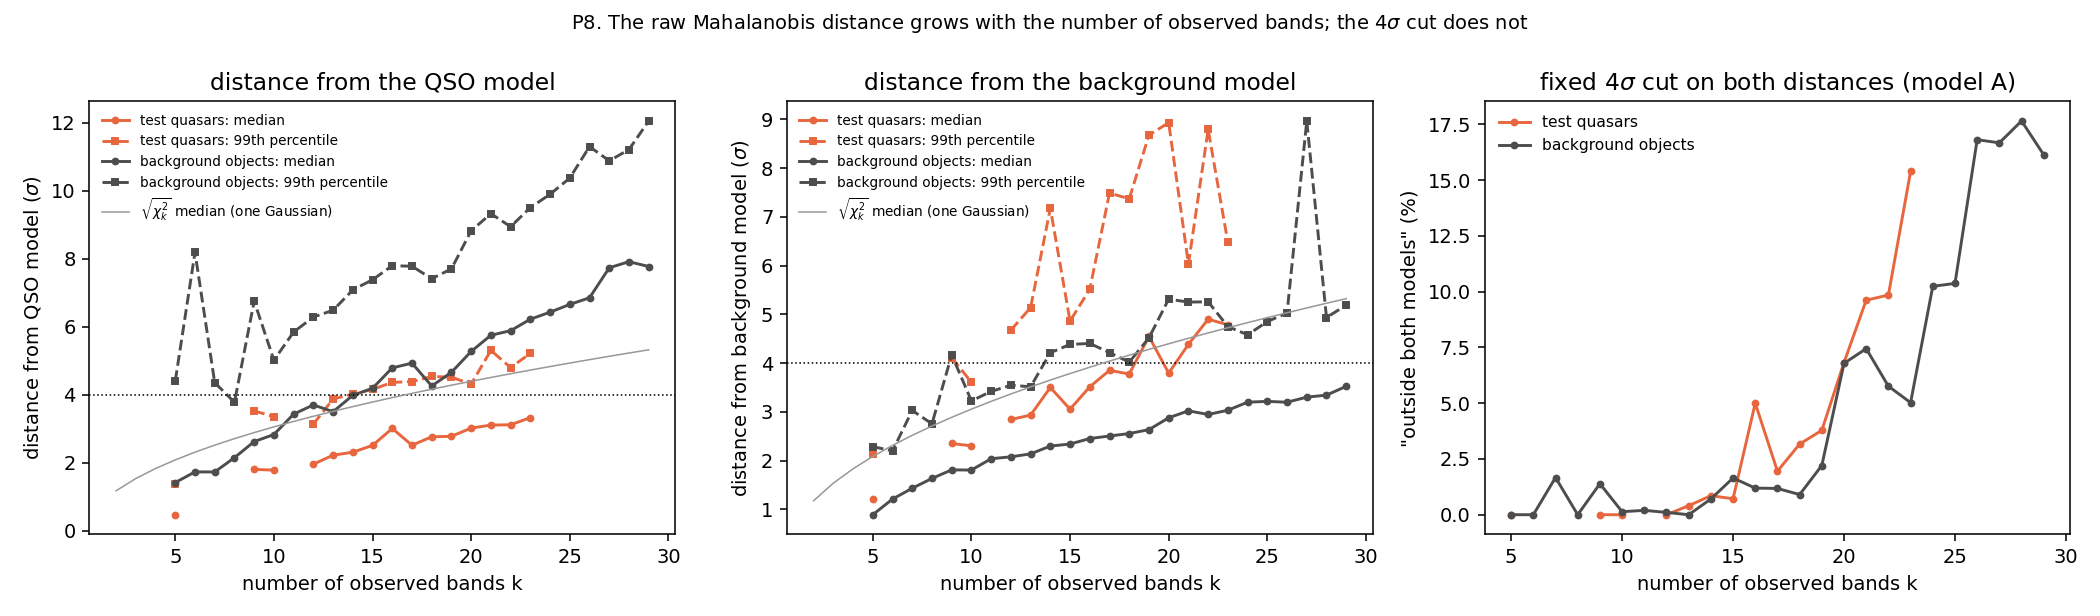
\includegraphics[width=\textwidth]{P8_distance_vs_bands.png}
\caption{Left and middle: median and 99th percentile of the distance from the quasar model ($d_Q$) and from the
background model ($d_B$) against the number of observed bands $k$, for test quasars (orange) and background
objects (dark grey), model A. Grey line: median of $\sqrt{\chi^2_k}$ for a single Gaussian. Dotted: the
$4\sigma$ cut. Right: fraction outside both models against $k$. Values of $k$ with fewer than 30 objects are
omitted.}
\label{fig:k}
\end{figure}

\subsection{Colours}
Figure~\ref{fig:col} overlays the unranked quasars (model A) on the colour distribution of the ranked ones in
four redshift ranges. Most unranked quasars lie inside or at the edge of the ranked distribution in every Legacy
colour plane; a minority are genuinely unusual (very red $g-r$ or $r-z$, which suggests dust reddening, or
very blue $z-W1$). This agrees with the distance picture: in a few colours they look ordinary, and they are
pushed past the cut by many small deviations across many bands.

\begin{figure}[H]\centering
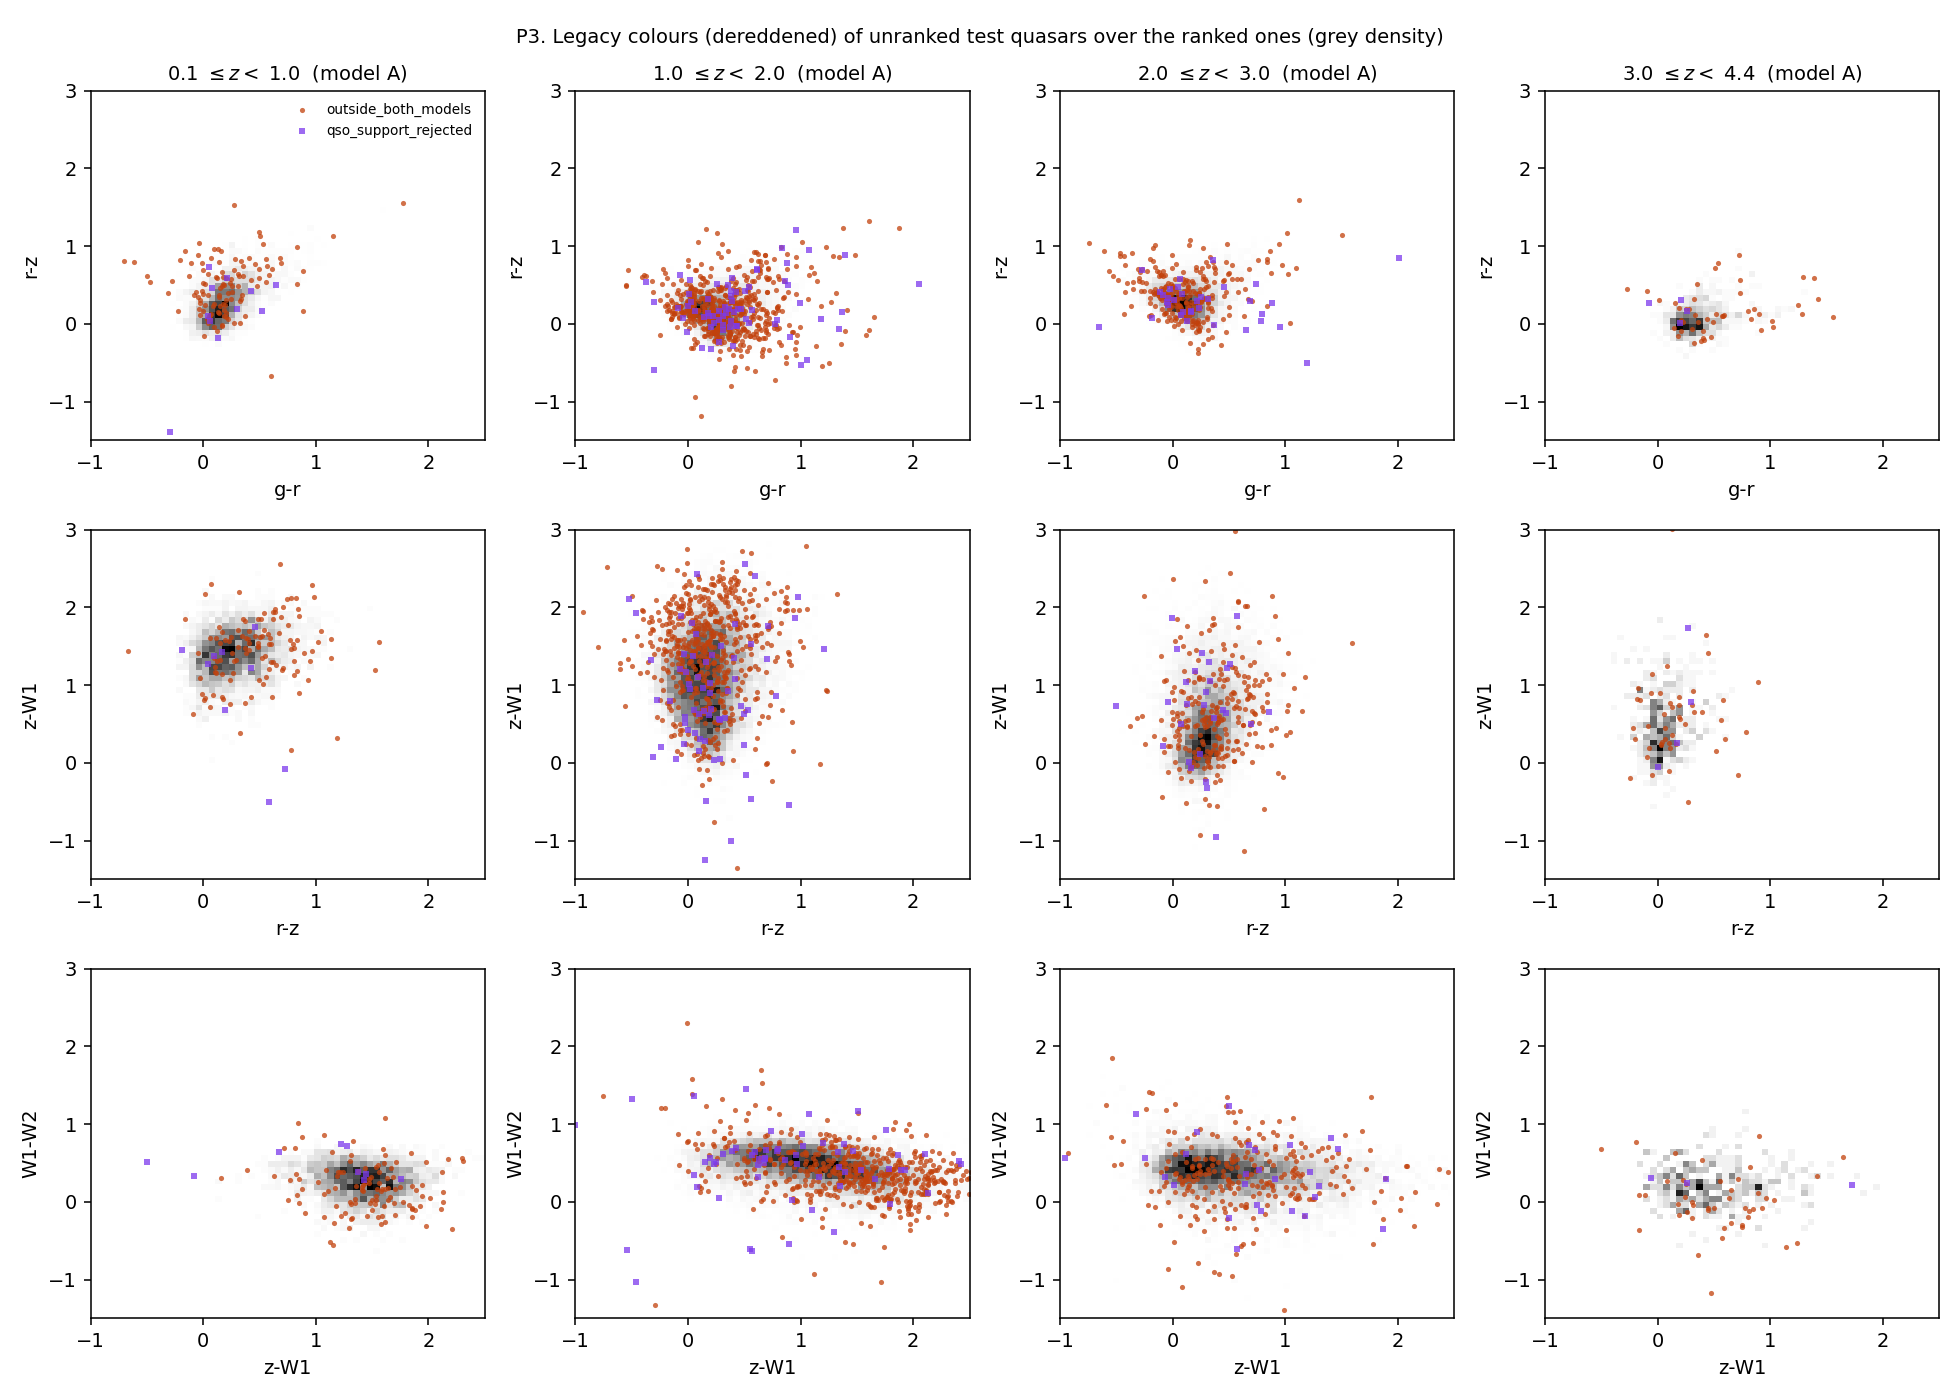
\includegraphics[width=\textwidth]{P3_unranked_colours.png}
\caption{Legacy colours (dereddened luptitudes) of unranked test quasars (orange: outside both models; purple:
support-rejected) over the density of ranked test quasars (grey), in four redshift ranges, model A.}
\label{fig:col}
\end{figure}

\subsection{Bands and surveys}
\paragraph{No single bad band.} Under the quasar model at each quasar's redshift (conditional on Legacy $r$), we
computed the standardised residual of every observed band (Fig.~\ref{fig:band}). Only 1--3.5\% of the unranked
quasars' bands deviate by more than $4\sigma$, spread over SDSS, Legacy, AllWISE and PS1 with no dominant band;
84\% (A) and 87\% (B) of the unranked quasars have no band beyond $4\sigma$ at all (ranked: 99\%). Their largest
single residual is typically 2--3$\sigma$, against 1--2$\sigma$ for ranked quasars.

\begin{figure}[H]\centering
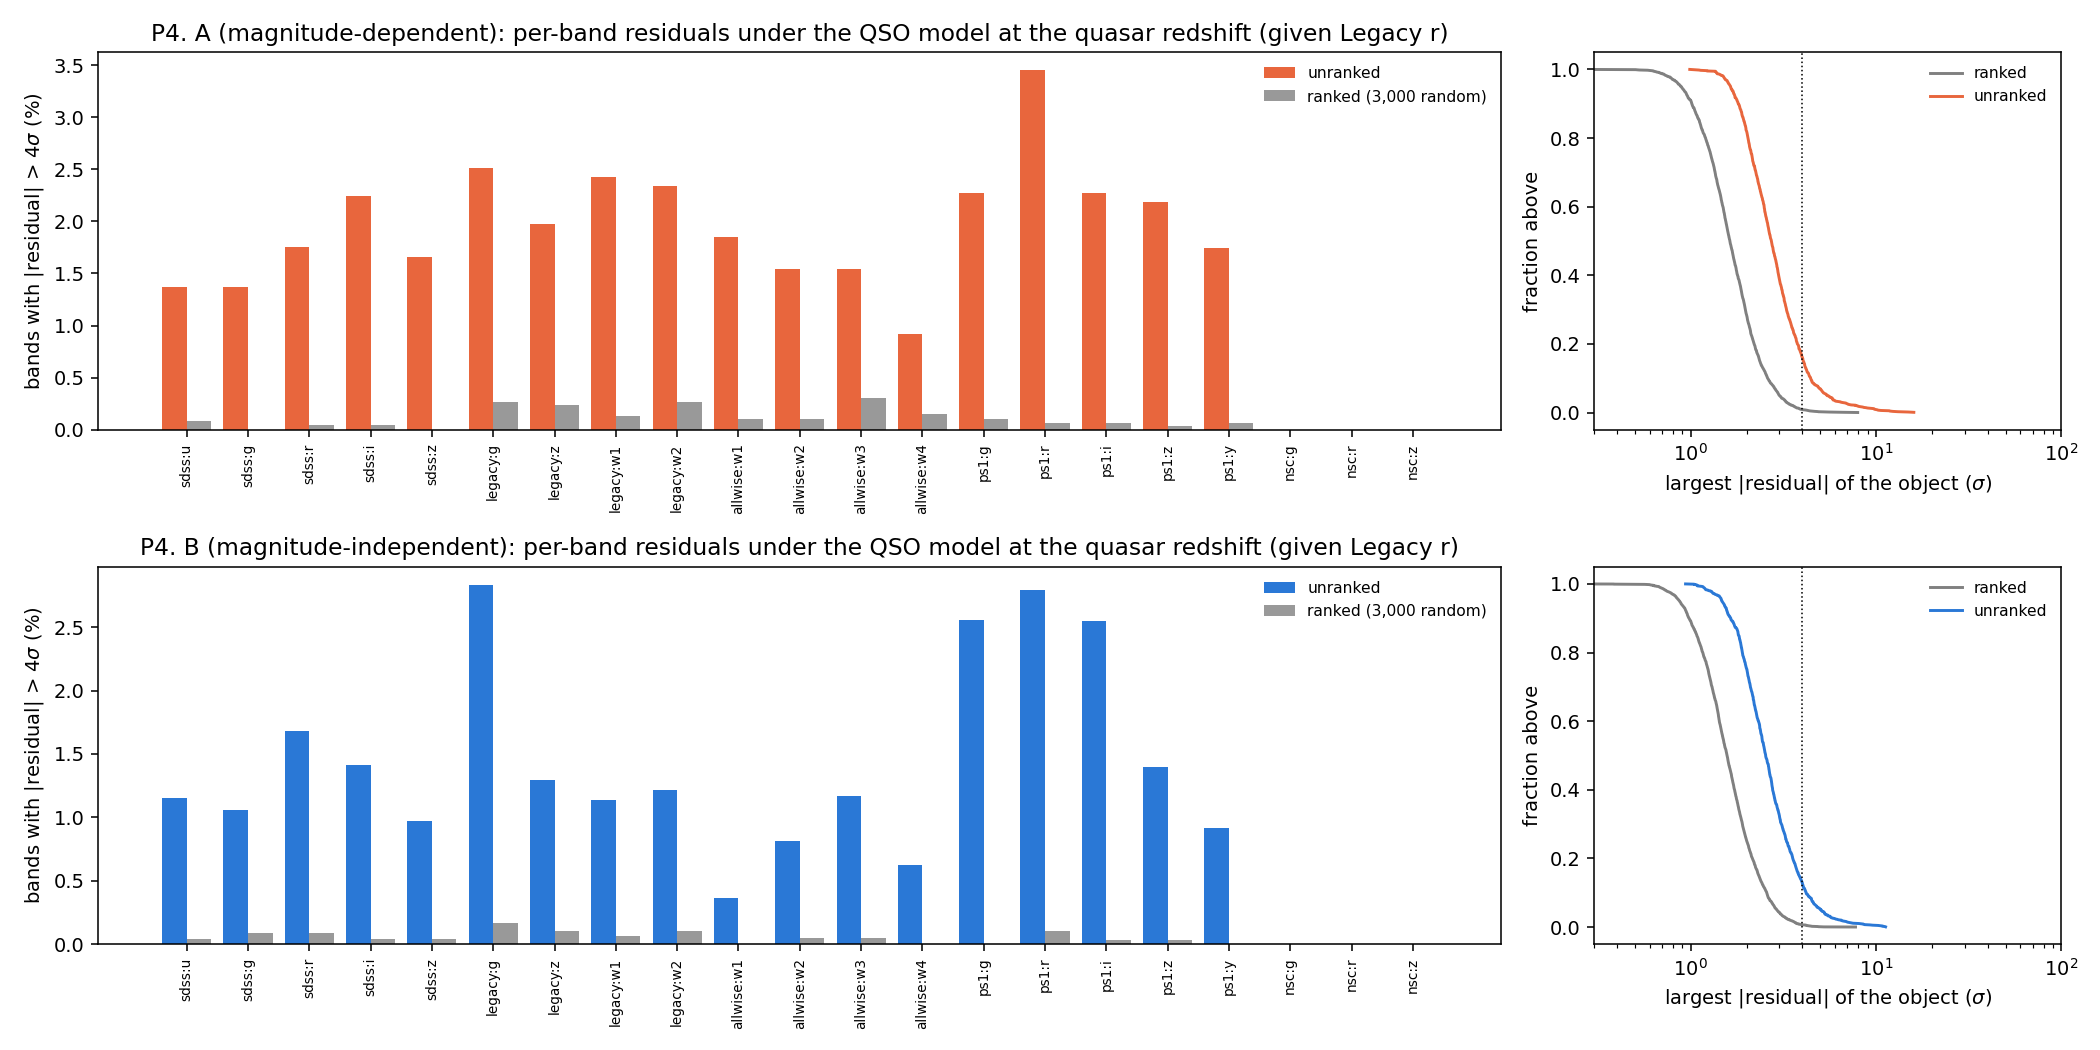
\includegraphics[width=\textwidth]{P4_band_residuals.png}
\caption{Left: percentage of observed bands with standardised residual $|R|>4$ under the quasar model at the
quasar's redshift, given Legacy $r$, for unranked quasars and 3,000 random ranked ones, by band (Legacy north and
south combined). Right: distribution of each object's largest $|R|$. Top: model A; bottom: model B.}
\label{fig:band}
\end{figure}

\paragraph{Survey-to-survey disagreement.} The surveys observed at different epochs and calibrate differently.
Figure~\ref{fig:surv} compares each quasar's SDSS and PS1 $r$ with its Legacy $r$. The unranked quasars have much
broader differences: $|r_{\rm SDSS}-r_{\rm Legacy}|>0.5$\,mag for 33\% of them (ranked: 11\%), and
$|r_{\rm PS1}-r_{\rm Legacy}|>0.5$\,mag for 28\% (ranked: 9\%). Quasar variability over the years between the surveys
(SDSS imaging 2000--2008, PS1 2010--2014, Legacy DR9 2014--2019) is the natural explanation; the model treats the surveys as simultaneous. Unranked quasars also more often
have SDSS (92\% against 78\%) and AllWISE (88\% against 66\%) photometry, i.e.\ more bands.

\begin{figure}[H]\centering
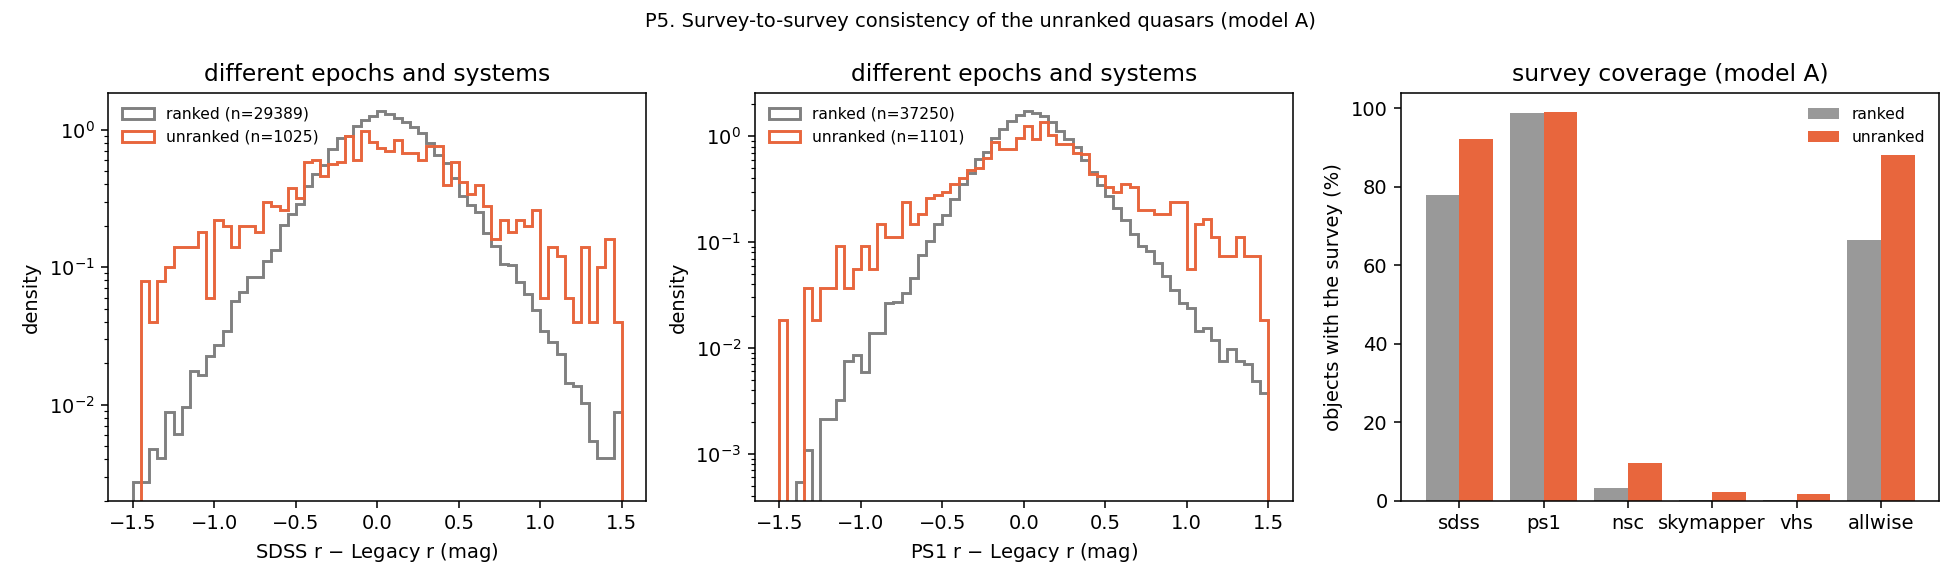
\includegraphics[width=\textwidth]{P5_survey_consistency.png}
\caption{Left and middle: SDSS $r$ and PS1 $r$ minus Legacy $r$ (dereddened luptitudes) for ranked (grey) and
unranked (orange) test quasars, model A. Right: fraction of each group with photometry from each survey.}
\label{fig:surv}
\end{figure}

\paragraph{Removing surveys.} We rescored the unranked quasars of each model with Legacy bands only, and with each
survey removed in turn (Fig.~\ref{fig:resc}). Rescoring with all bands reproduces the original result (none
ranked). With Legacy $g,r,z,W1,W2$ only, 93\% (A) and 94\% (B) are ranked. Removing SDSS ranks 78--79\%, PS1
80--85\%, AllWISE 70--75\% and the Legacy WISE bands 56--57\%; removing NSC, SkyMapper or VHS ranks 0.6--6\%,
because few of these quasars have them. That removing \emph{any} large survey rescues most of them, rather than one
specific survey, is the signature of the dimension effect, with variability between epochs adding to it.

\begin{figure}[H]\centering
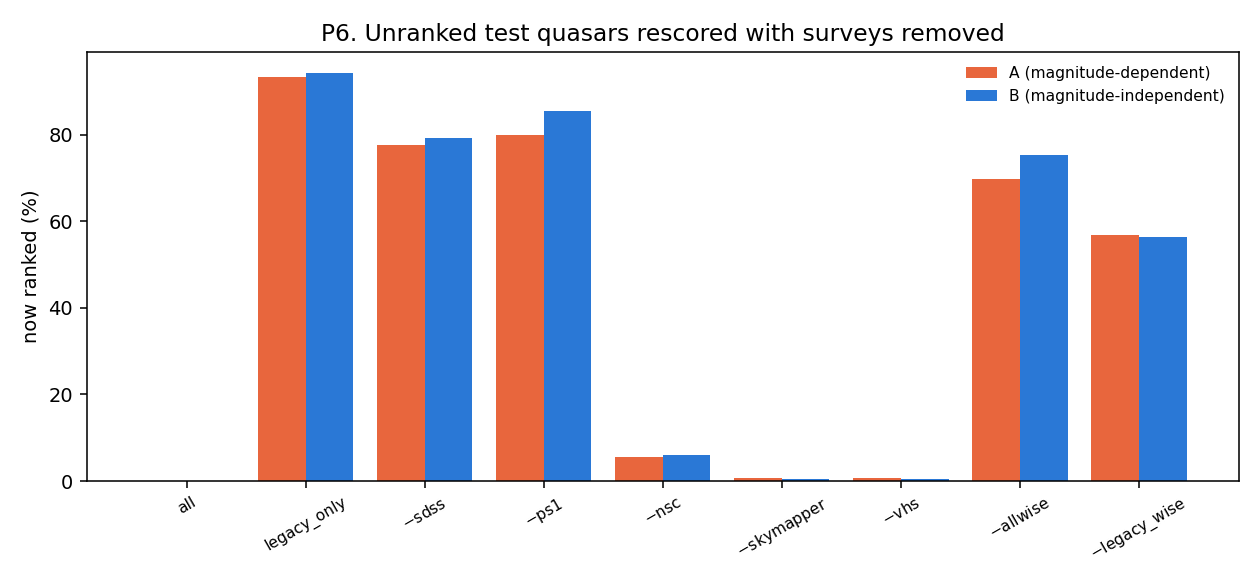
\includegraphics[width=0.75\textwidth]{P6_rescore_surveys.png}
\caption{Unranked test quasars rescored with surveys removed: percentage now ranked, for models A and B.
``all'': no band removed (reproduces the original); ``legacy\_only'': Legacy $g,r,z,W1,W2$ only; ``$-$survey'':
that survey's bands removed.}
\label{fig:resc}
\end{figure}

\subsection{What to do}
\begin{enumerate}
\item \textbf{Make the outside-both-models threshold depend on the number of observed bands.} Calibrate
  $t(k)$ empirically on calibration-role objects (not the test set), for example so that a fixed small fraction
  (say 0.2\%) of calibration quasars and of calibration background objects lie beyond it at each $k$, pooling
  sparse $k$. The $\chi^2_k$ form is the wrong shape (it overshoots), but a scaled version may fit. Background
  objects cross the fixed cut in the same way (Fig.~\ref{fig:k}), so the change affects their abstention too; the
  AUC and the incidence of background objects at high $\pq$ must be re-measured on the test set afterwards.
\item \textbf{Consider an inter-survey variability term}: an extra, magnitude- and time-baseline-dependent
  variance between surveys observed at different epochs, at least for quasars. This addresses the secondary cause
  and is a larger change to the model.
\item Until then: an unranked object with many bands is not evidence against a quasar. Rescoring it with Legacy
  bands only is a valid check; 93--94\% of the unranked test quasars are ranked that way.
\end{enumerate}

\subsection{The fix: a calibrated outside-both-models test}\label{sec:fix}
Implemented in \code{qso\_pcolor.ood\_calibration} and available in the scorer as
\code{ood\_calibration=dict(alpha, draws, seed)}; the default of \code{UnifiedPSFModel.score} since 5 October 2026. The statistic is unchanged: the
squared nearest-component distance $T_c$ of the non-reference bands given Legacy $r$, with the object's noise
added, for the quasar model (all redshift slices, equal weight) and for the background model (weights at the
object's sky position). For each object we draw 256 members of each class model conditioned on the object's own
$r$, in its own observed bands and with its own noise, compute the same statistic, and form
\[
p_c=\frac{1+\#\{T_c^{\rm fake}\ge T_c^{\rm obs}\}}{257}.
\]
The object is outside both models when $p_Q<\alpha$ and $p_B<\alpha$, with $\alpha=2/256$ set in advance (as for
the support cut). This is a parametric-bootstrap tail probability of the existing statistic, so it handles the
number and the identity of the observed bands, the noise and the nearest-of-many-components effect at once. It costs
13\,ms per object for both models. Unit tests check that $p$ is uniform for members of a known mixture in 4, 12 and
25 dimensions (where the raw distance of a typical member exceeds $3\sigma$), and that the scorer path reproduces
the offline values and is independent of batch order.

\paragraph{Calibration role (a-priori check of $\alpha$).} On 4,000 calibration-role quasars and 4,000 background
objects, the new test flags 0.23--0.25\% of quasars and 0.48--0.60\% of background objects; a class member falls
below $\alpha$ in its own model in 0.4\% (quasars) and 0.75\% (background) of cases, against the nominal 0.78\%.

\paragraph{Test panel.} Figure~\ref{fig:fix} and the table compare the two rules on the held-out panel
(38,881 quasars, 14,247 background objects). The objects whose flag clears were rescored through the scorer.
\begin{center}\small
\begin{tabular}{lcccc}
\toprule
& \multicolumn{2}{c}{A (magnitude-dependent)} & \multicolumn{2}{c}{B (magnitude-independent)} \\
& fixed $4\sigma$ & calibrated & fixed $4\sigma$ & calibrated \\
\midrule
Quasars outside both models & 2.54\% & 0.14\% & 2.91\% & 0.17\% \\
Quasars unranked (all reasons) & 2.86\% & 0.61\% & 3.18\% & 0.57\% \\
Background outside both models & 2.09\% & 0.51\% & 2.14\% & 0.53\% \\
Background unranked (all reasons) & 69.2\% & 69.1\% & 59.9\% & 59.7\% \\
Quasar recall ($\pq>0.5$) & 0.891 & 0.913 & 0.859 & 0.883 \\
Background incidence ($\pq>0.5$) & 1.14\% & 1.19\% & 1.08\% & 1.14\% \\
AUC ($\log\mathcal{R}$, unranked at the bottom) & 0.980 & 0.994 & 0.976 & 0.994 \\
\bottomrule
\end{tabular}
\end{center}
The refusal rate no longer depends on the number of bands, for quasars or background objects. Of the 947 (A) and
1,079 (B) quasars whose flag clears, 93--95\% are then ranked; the rest fail the support cut. Only 7 (A) and 9 (B)
quasars are newly flagged. Almost all background objects whose flag clears (245 of 263, A) are still not ranked,
because the support cut catches them, so background incidence rises by only 0.05--0.06 percentage points (7--8 of 14,247
objects). The AUC rises by 0.014--0.018 because the AUC as defined counts an unranked quasar as ranked
below every ranked background object and tied with the unranked ones: moving 2.3--2.6\% of quasars from the bottom
to their scores accounts for the change. The real quasars' $p_Q$ values lie below the uniform line
(Fig.~\ref{fig:fix}, right): the quasar model is, if anything, slightly broad, so the test is conservative.

\begin{figure}[H]\centering
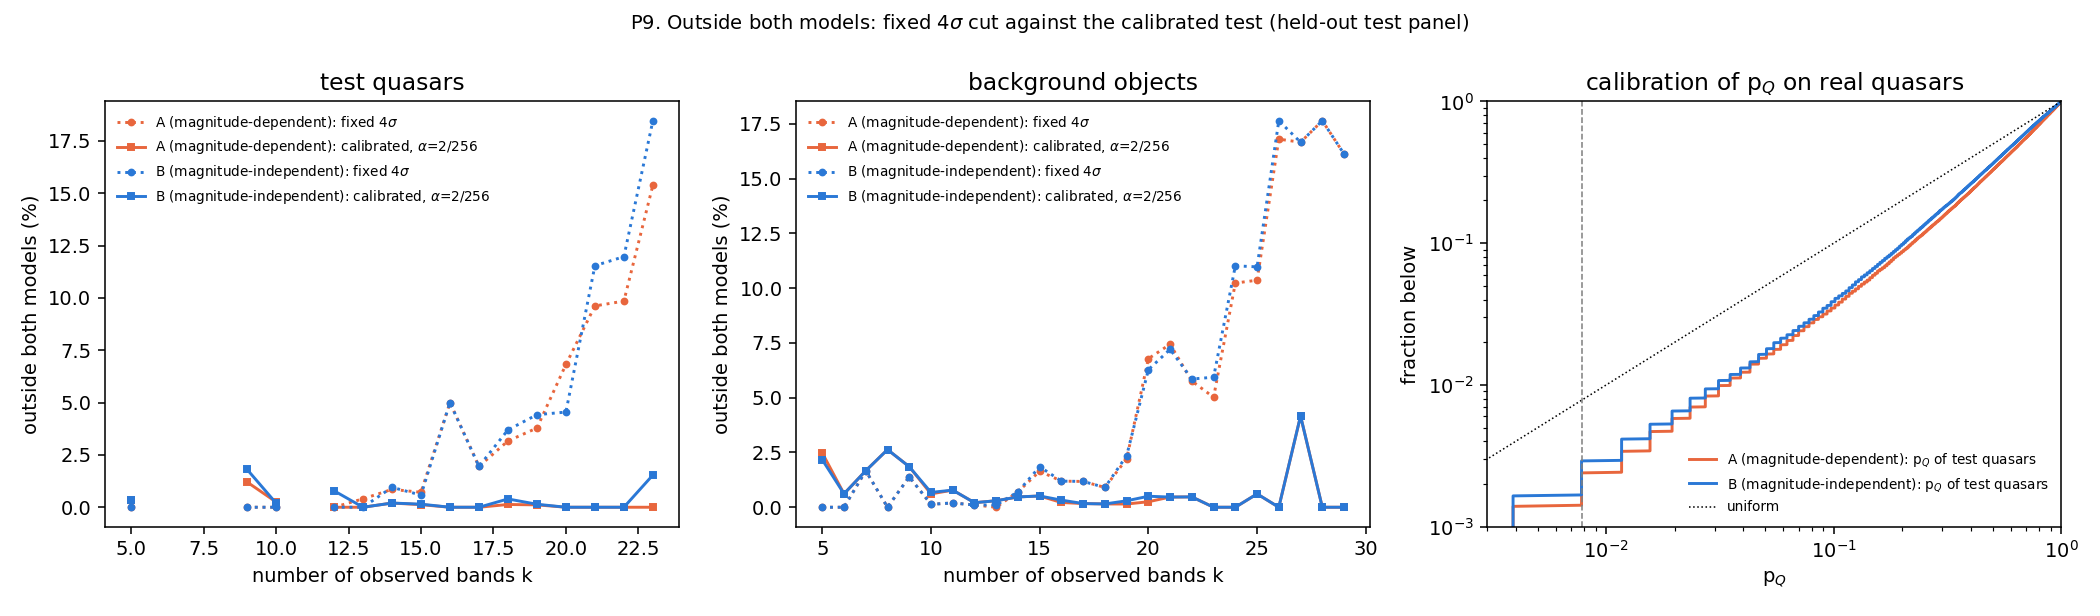
\includegraphics[width=\textwidth]{P9_calibrated_ood.png}
\caption{Outside-both-models fraction against the number of observed bands for the fixed $4\sigma$ cut (dotted) and
the calibrated test with $\alpha=2/256$ (solid), for test quasars (left) and background objects (middle), models A
and B. Right: cumulative distribution of $p_Q$ for the test quasars (dotted: uniform; dashed: $\alpha$).}
\label{fig:fix}
\end{figure}

%======================================================================
\section{Part 2: overconfidence at the top}
%======================================================================
\subsection{Reliability above $\pq=0.5$}
Among ranked objects of the natural population we bin $\pq$ and count known quasars, flagged background objects
and unflagged background objects (each background object weighted by 2.75). The observed quasar fraction is
bracketed by a lower bound (only known quasars count) and an upper bound (flagged background objects also count).

\begin{center}\small
\begin{tabular}{lrrrrcc}
\toprule
$\pq$ bin & mean $\pq$ & known QSOs & flagged bkg & unflagged bkg & lower & upper \\
\midrule
\multicolumn{7}{l}{\emph{Model A}} \\
0.90--0.95 & 0.926 & 82 & 28 & 6 & 0.47 & 0.91 \\
0.95--0.97 & 0.961 & 42 & 13 & 3 & 0.49 & 0.90 \\
0.97--0.99 & 0.982 & 122 & 28 & 4 & 0.58 & 0.95 \\
0.99--0.999 & 0.996 & 213 & 42 & 8 & 0.61 & 0.94 \\
$>0.999$ & 1.000 & 755 & 101 & 5 & 0.72 & 0.99 \\
\multicolumn{7}{l}{\emph{Model B}} \\
0.90--0.95 & 0.929 & 74 & 23 & 3 & 0.51 & 0.94 \\
0.95--0.97 & 0.961 & 48 & 13 & 2 & 0.54 & 0.94 \\
0.97--0.99 & 0.982 & 127 & 21 & 5 & 0.64 & 0.93 \\
0.99--0.999 & 0.996 & 206 & 36 & 6 & 0.64 & 0.95 \\
$>0.999$ & 1.000 & 704 & 102 & 6 & 0.70 & 0.98 \\
\bottomrule
\end{tabular}
\end{center}
Background counts are unweighted; the bounds use the weight. At $\pq>0.9$ the upper bound is 0.01--0.06 below the mean
prediction, and the lower bound 0.28--0.47 below it (Fig.~\ref{fig:top}, left).

\subsection{Who the high-$\pq$ background objects are}
With model A, 188 background objects have $\pq>0.97$. 171 (91\%) are flagged as likely quasars: 118 by WISE colour
alone, 36 by WISE colour with Gaia astrometry consistent with zero proper motion, and 17 by Quaia membership (all
also WISE-flagged). Only 17 are unflagged (16 with no flag of any kind, one with only the zero-proper-motion
diagnostic, which is not part of the flag). Their magnitudes are those of the high-$\pq$ known quasars (median
$r=21.2$ against 20.7), and in $W1-W2$ they lie with the known quasars, above the stellar locus
(Fig.~\ref{fig:top}, middle and right). The WISE flag requires $S/N\ge5$ in both $W1$ and $W2$. Of the 17 unflagged objects, 3 have $W1-W2$ above the
AGN threshold but $W2$ $S/N<5$, 4 more have too little $W1$ or $W2$ signal for a reliable colour, and 10 have
stellar-like $W1-W2$ ($-0.3$ to $+0.13$ AB, several close to the threshold of 0.16) with good $S/N$. These 10
are the plausible genuine contaminants. After weighting, all 17 unflagged objects are 2.9\% of the objects at
$\pq>0.97$, and the 10 with stellar infrared colours 1.7\%.

\begin{figure}[H]\centering
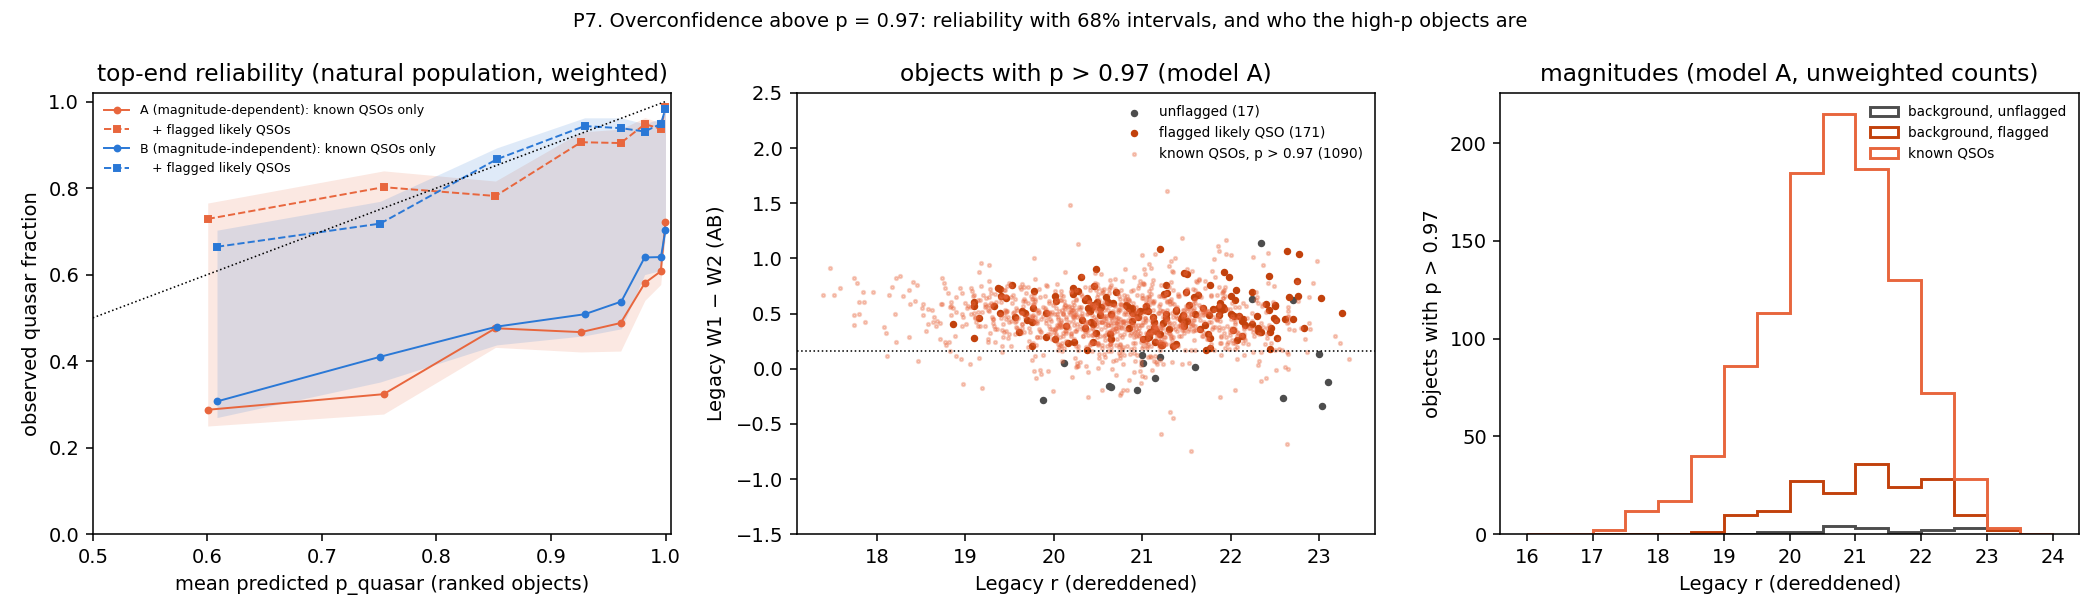
\includegraphics[width=\textwidth]{P7_top_end.png}
\caption{Left: observed quasar fraction against mean predicted $\pq$ for ranked objects of the natural test-cone
population, counting known quasars only (solid, lower bound) or also flagged likely quasars (dashed, upper bound);
shading: 68\% Wilson intervals of the two bounds. Middle: Legacy $W1-W2$ (AB) against $r$ for objects with
$\pq>0.97$ under model A: known quasars (light), flagged background objects (dark orange) and unflagged ones
(black). Dotted: the WISE AGN threshold ($W1-W2=0.8$ Vega). Right: their $r$ distributions (unweighted).}
\label{fig:top}
\end{figure}

\subsection{Interpretation}
The apparent overconfidence of the method note (``$\pq>0.99$ gives 0.69--0.98 observed'') is mostly a property of
the labels. The background sample is a photometric catalogue with known quasars removed; it still contains
quasars that have no spectrum, and the objects the model is most confident about are exactly those. If the
flagged objects are quasars, the top end is calibrated to within a few per cent; the unflagged objects
bound the genuine contamination at 1.7--2.9\% at $\pq>0.97$ (more if some flagged objects are not quasars). A recalibration fitted
to the lower-bound labels would make the model \emph{under}confident on real quasars, which is why none was
applied. The ranking is unaffected either way.

\paragraph{What would settle it.} Spectroscopic labels for the flagged objects: cross-matching them with DESI DR1
spectra not used as training labels, or a newer release, would move the lower bound towards the upper. With 171
high-$\pq$ flagged objects in the test cones, a few dozen spectra would already measure the fraction.

\section{Conclusions}
\begin{itemize}
\item The 2.9--3.2\% of real quasars left unranked are mainly an artefact of a fixed $4\sigma$ cut on a distance
  that grows with the number of observed bands. They are ordinary quasars with many bands, plus a smaller
  contribution from variability between surveys. The calibrated test (Section~\ref{sec:fix}) recovers 80\% of
  them without raising background incidence, and is now the default.
\item The top-end overconfidence is mostly unlabelled quasars in the background sample. The model's highest
  probabilities are consistent with the upper label bound; unflagged background objects make up 1.7--2.9\% of
  the objects at $\pq>0.97$.
\end{itemize}

\end{document}
